
% This LaTeX was auto-generated from MATLAB code.
% To make changes, update the MATLAB code and republish this document.











    
    \begin{DoxyCode}
function example_dirac_secondorder()
\end{DoxyCode}
\begin{par}
COMPILATION
\end{par} \vspace{1em}
\begin{DoxyCode}
    [exdir,~,~]=fileparts(which('example_dirac_secondorder.m'));
    % compile the model
    amiwrap('model_dirac_secondorder','model_dirac_secondorder_syms',exdir,1)
\end{DoxyCode}

         \begin{DoxyCode}Generating model struct ...
x | k | p | deltax | xdot | deltaxdot | ddeltaxdx | ddeltaxdp | ddeltaxdt | root | drootdx | sx | drootdp | drootdt | dtaudp | sroot | stau | deltasx | sigma_y | dsigma_ydp | y | dydp | sigma_z | dsigma_zdp | z | dzdp | Parsing model struct ...
z | 

Generating C code ...
deltasx | deltax | dsigma_ydp | dsigma_zdp | dydp | dzdp | root | sigma_y | sigma_z | stau | xdot | y | z | headers | wrapfunctions | 
headers | wrapfunctions | 
Compiling mex file ...
amici | Building with 'Xcode with Clang'.
MEX completed successfully.
Building with 'Xcode with Clang'.
MEX completed successfully.
amici | Building with 'Xcode with Clang'.
MEX completed successfully.
Building with 'Xcode with Clang'.
MEX completed successfully.
\end{DoxyCode} 
    \begin{par}
SIMULATION
\end{par} \vspace{1em}
\begin{DoxyCode}
    % time vector
    t = linspace(0,3,1001);
    p = [1;0.5;2;3];
    k = [];

    options = amioption('sensi',0,...
        'maxsteps',1e4);

    % load mex into memory
    [msg] = which('simulate_model_secondorder_dirac'); % fix for inaccessability problems
    options.sensi = 2;
    sol = simulate_model_dirac_secondorder(t,log10(p),k,[],options);
\end{DoxyCode}
\begin{par}
FORWARD SENSITIVITY ANALYSIS
\end{par} \vspace{1em}
\begin{DoxyCode}
    options.sensi = 2;

    sol = simulate_model_dirac_secondorder(t,log10(p),k,[],options);
\end{DoxyCode}
\begin{par}
FINITE DIFFERENCES
\end{par} \vspace{1em}
\begin{DoxyCode}
    options.sensi = 1;

    eps = 1e-4;
    xi = log10(p);
    for ip = 1:4;
        xip = xi;
        xip(ip) = xip(ip) + eps;
        solp = simulate_model_dirac_secondorder(t,xip,k,[],options);
        s2x_fd(:,:,:,ip) = (solp.sx - sol.sx)/eps;
        s2y_fd(:,:,:,ip) = (solp.sy - sol.sy)/eps;
    end
\end{DoxyCode}
\begin{par}
PLOTTING
\end{par} \vspace{1em}
\begin{DoxyCode}
    figure
    c_x = get(gca,'ColorOrder');
    for ip = 1:4
        for jp = 1:4
            subplot(4,4,(ip-1)*4+jp)
            hold on
            for ix = 1:size(sol.x,2)
                plot(t,sol.s2x(:,ix,ip,jp),'.-','Color',c_x(ix,:))
                plot(t,s2x_fd(:,ix,ip,jp),'--','Color',c_x(ix,:))
            end
            ylim([-10,10])
            legend('x1','x1_{fd}','x2','x2_{fd}','Location','NorthEastOutside')
            legend boxoff
            title(['state sensitivity for p' num2str(ip) '/p' num2str(jp)])
            xlabel('time t')
            ylabel('x')
            box on
        end
    end
    set(gcf,'Position',[100 300 1200 500])
    figure
    for ip = 1:4
        for jp = 1:4
            subplot(4,4,(ip-1)*4+jp)
            plot(t,abs(sol.s2x(:,:,ip,jp)-s2x_fd(:,:,ip,jp)),'r--')
            legend('error x1','error x2','Location','NorthEastOutside')
            legend boxoff
            title(['state sensitivity for p' num2str(ip) '/p' num2str(jp)])
            xlabel('time t')
            ylabel('error')
            ylim([1e-12,1e0])
            set(gca,'YScale','log')
            box on
        end
    end
    set(gcf,'Position',[100 300 1200 500])

    drawnow
\end{DoxyCode}

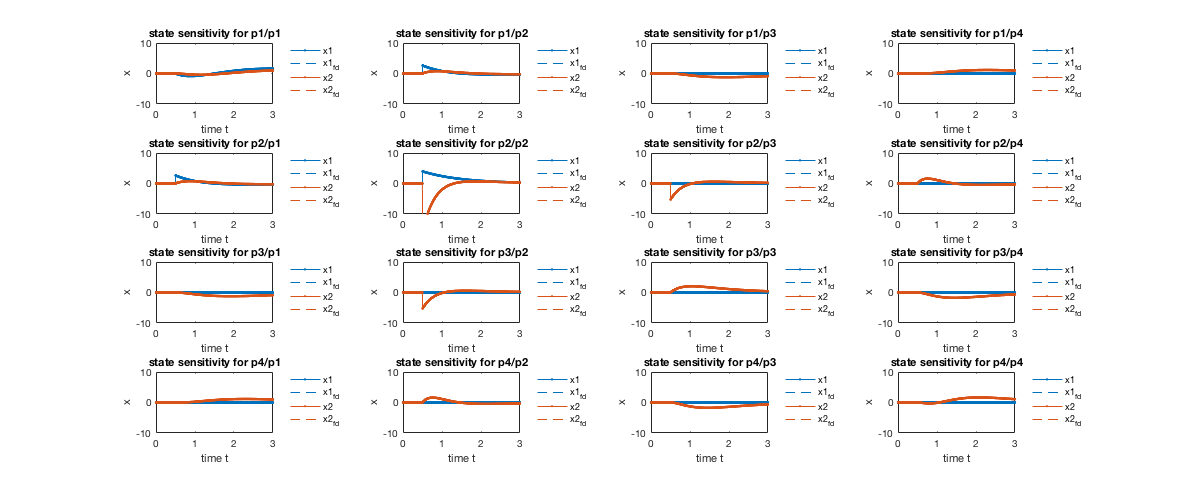
\includegraphics[width=\textwidth]{../../examples/example_dirac_secondorder/html/example_dirac_secondorder_01.png}

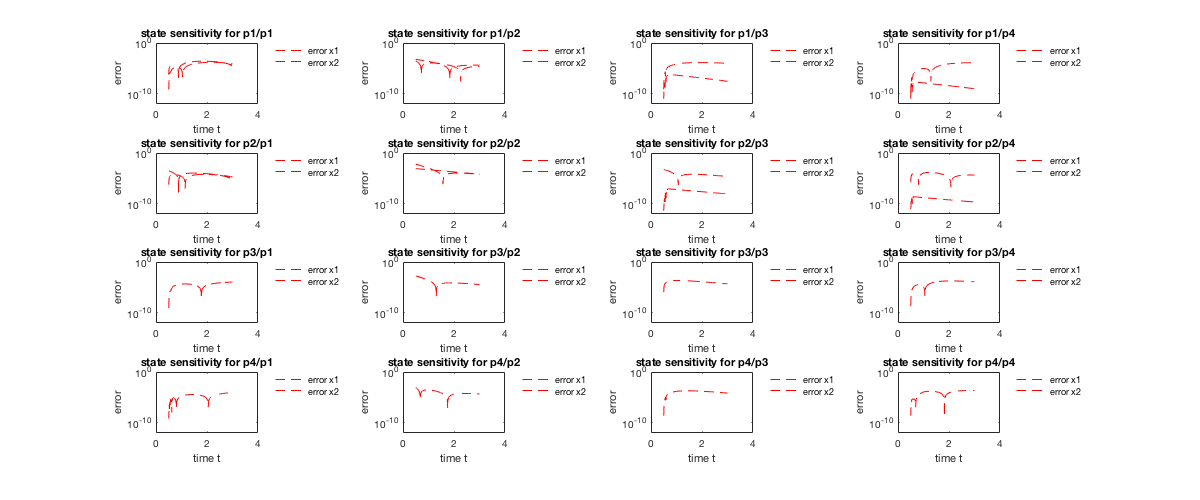
\includegraphics[width=\textwidth]{../../examples/example_dirac_secondorder/html/example_dirac_secondorder_02.png}
\begin{DoxyCode}
end
\end{DoxyCode}




    